% Options for packages loaded elsewhere
\PassOptionsToPackage{unicode}{hyperref}
\PassOptionsToPackage{hyphens}{url}
%
\documentclass[
]{article}
\usepackage{amsmath,amssymb}
\usepackage{lmodern}
\usepackage{iftex}
\ifPDFTeX
  \usepackage[T1]{fontenc}
  \usepackage[utf8]{inputenc}
  \usepackage{textcomp} % provide euro and other symbols
\else % if luatex or xetex
  \usepackage{unicode-math}
  \defaultfontfeatures{Scale=MatchLowercase}
  \defaultfontfeatures[\rmfamily]{Ligatures=TeX,Scale=1}
\fi
% Use upquote if available, for straight quotes in verbatim environments
\IfFileExists{upquote.sty}{\usepackage{upquote}}{}
\IfFileExists{microtype.sty}{% use microtype if available
  \usepackage[]{microtype}
  \UseMicrotypeSet[protrusion]{basicmath} % disable protrusion for tt fonts
}{}
\makeatletter
\@ifundefined{KOMAClassName}{% if non-KOMA class
  \IfFileExists{parskip.sty}{%
    \usepackage{parskip}
  }{% else
    \setlength{\parindent}{0pt}
    \setlength{\parskip}{6pt plus 2pt minus 1pt}}
}{% if KOMA class
  \KOMAoptions{parskip=half}}
\makeatother
\usepackage{xcolor}
\usepackage[margin=1in]{geometry}
\usepackage{longtable,booktabs,array}
\usepackage{calc} % for calculating minipage widths
% Correct order of tables after \paragraph or \subparagraph
\usepackage{etoolbox}
\makeatletter
\patchcmd\longtable{\par}{\if@noskipsec\mbox{}\fi\par}{}{}
\makeatother
% Allow footnotes in longtable head/foot
\IfFileExists{footnotehyper.sty}{\usepackage{footnotehyper}}{\usepackage{footnote}}
\makesavenoteenv{longtable}
\usepackage{graphicx}
\makeatletter
\def\maxwidth{\ifdim\Gin@nat@width>\linewidth\linewidth\else\Gin@nat@width\fi}
\def\maxheight{\ifdim\Gin@nat@height>\textheight\textheight\else\Gin@nat@height\fi}
\makeatother
% Scale images if necessary, so that they will not overflow the page
% margins by default, and it is still possible to overwrite the defaults
% using explicit options in \includegraphics[width, height, ...]{}
\setkeys{Gin}{width=\maxwidth,height=\maxheight,keepaspectratio}
% Set default figure placement to htbp
\makeatletter
\def\fps@figure{htbp}
\makeatother
\setlength{\emergencystretch}{3em} % prevent overfull lines
\providecommand{\tightlist}{%
  \setlength{\itemsep}{0pt}\setlength{\parskip}{0pt}}
\setcounter{secnumdepth}{5}
\newlength{\cslhangindent}
\setlength{\cslhangindent}{1.5em}
\newlength{\csllabelwidth}
\setlength{\csllabelwidth}{3em}
\newlength{\cslentryspacingunit} % times entry-spacing
\setlength{\cslentryspacingunit}{\parskip}
\newenvironment{CSLReferences}[2] % #1 hanging-ident, #2 entry spacing
 {% don't indent paragraphs
  \setlength{\parindent}{0pt}
  % turn on hanging indent if param 1 is 1
  \ifodd #1
  \let\oldpar\par
  \def\par{\hangindent=\cslhangindent\oldpar}
  \fi
  % set entry spacing
  \setlength{\parskip}{#2\cslentryspacingunit}
 }%
 {}
\usepackage{calc}
\newcommand{\CSLBlock}[1]{#1\hfill\break}
\newcommand{\CSLLeftMargin}[1]{\parbox[t]{\csllabelwidth}{#1}}
\newcommand{\CSLRightInline}[1]{\parbox[t]{\linewidth - \csllabelwidth}{#1}\break}
\newcommand{\CSLIndent}[1]{\hspace{\cslhangindent}#1}
\usepackage{subfig}
\usepackage{biblatex}
\addbibresource{references.bib}
\usepackage{booktabs}
\usepackage{longtable}
\usepackage{array}
\usepackage{multirow}
\usepackage{wrapfig}
\usepackage{float}
\usepackage{colortbl}
\usepackage{pdflscape}
\usepackage{tabu}
\usepackage{threeparttable}
\usepackage{threeparttablex}
\usepackage[normalem]{ulem}
\usepackage{makecell}
\usepackage{xcolor}
\ifLuaTeX
  \usepackage{selnolig}  % disable illegal ligatures
\fi
\IfFileExists{bookmark.sty}{\usepackage{bookmark}}{\usepackage{hyperref}}
\IfFileExists{xurl.sty}{\usepackage{xurl}}{} % add URL line breaks if available
\urlstyle{same} % disable monospaced font for URLs
\hypersetup{
  pdftitle={Heli-GPS Analysis in the Context of Mountain Pine Beetle},
  pdfauthor={Leonard Buechner},
  hidelinks,
  pdfcreator={LaTeX via pandoc}}

\title{Heli-GPS Analysis in the Context of Mountain Pine Beetle}
\author{Leonard Buechner}
\date{2022-04-27}

\begin{document}
\maketitle

{
\setcounter{tocdepth}{2}
\tableofcontents
}
\hypertarget{stratification}{%
\section{Stratification}\label{stratification}}

After lodgepole pines (Pinus contorta) have been attacked by Mountain Pine Beetle (MPB), they show different stages. The needles of attacked trees wil turn from green over yellow to red within the first 12 months (red-attack). It then takes in between 1-3 years until all needles have fallen to the ground, when the trees remain standing but without needles (grey-attack) (Wulder, White, and Dymond 2005). Depending on the type of stand, according to Mitchell and Preisler (1998), dead trees begin to fall after 3 to 5 years and 80 - 90 \% of trees had fallen after 11 years.
This leads to different stages of beetle attack that will be considered in this study. All green-attack trees detected in 2021 and 2020 are now with high probability in the red-attack stage. Some of the trees that have been detected as red-attack in 2021, will still classify as red-attack and others as grey-attack. A clear distinction based on time of detection is not possible without additional data, since it can take several years before all needles have fallen of the tree, the GPS locations of MPB-attacked trees provided by the government of Alberta (Wulder, White, and Dymond 2005). Collecting the LiDAR data at the end of May, all green-attack trees that have been attacked in 2019 and before, as well as all red-attack trees detected in 2020 and before, will now classify as grey attack. Additionally, it can be expected that most of the trees that have been detected as red-attack in 2011 and before, now have fallen to the ground (Schoennagel et al. 2012).

Three broad areas of interest have been selected (refer to fig.~\ref{fig:AoIs}) based on availability of observed MPB attacks in the years 2011, 2019, 2020, and 2021, while also having a dense network of paved roads and gravel roads. These areas of interest will be referred to as th Grande Prairie (GP) area in the North-West, the Whitecourt (WC) area in the North-East, and the Rocky Mountain House (RMH) area to the South-East.

\begin{figure}

{\centering 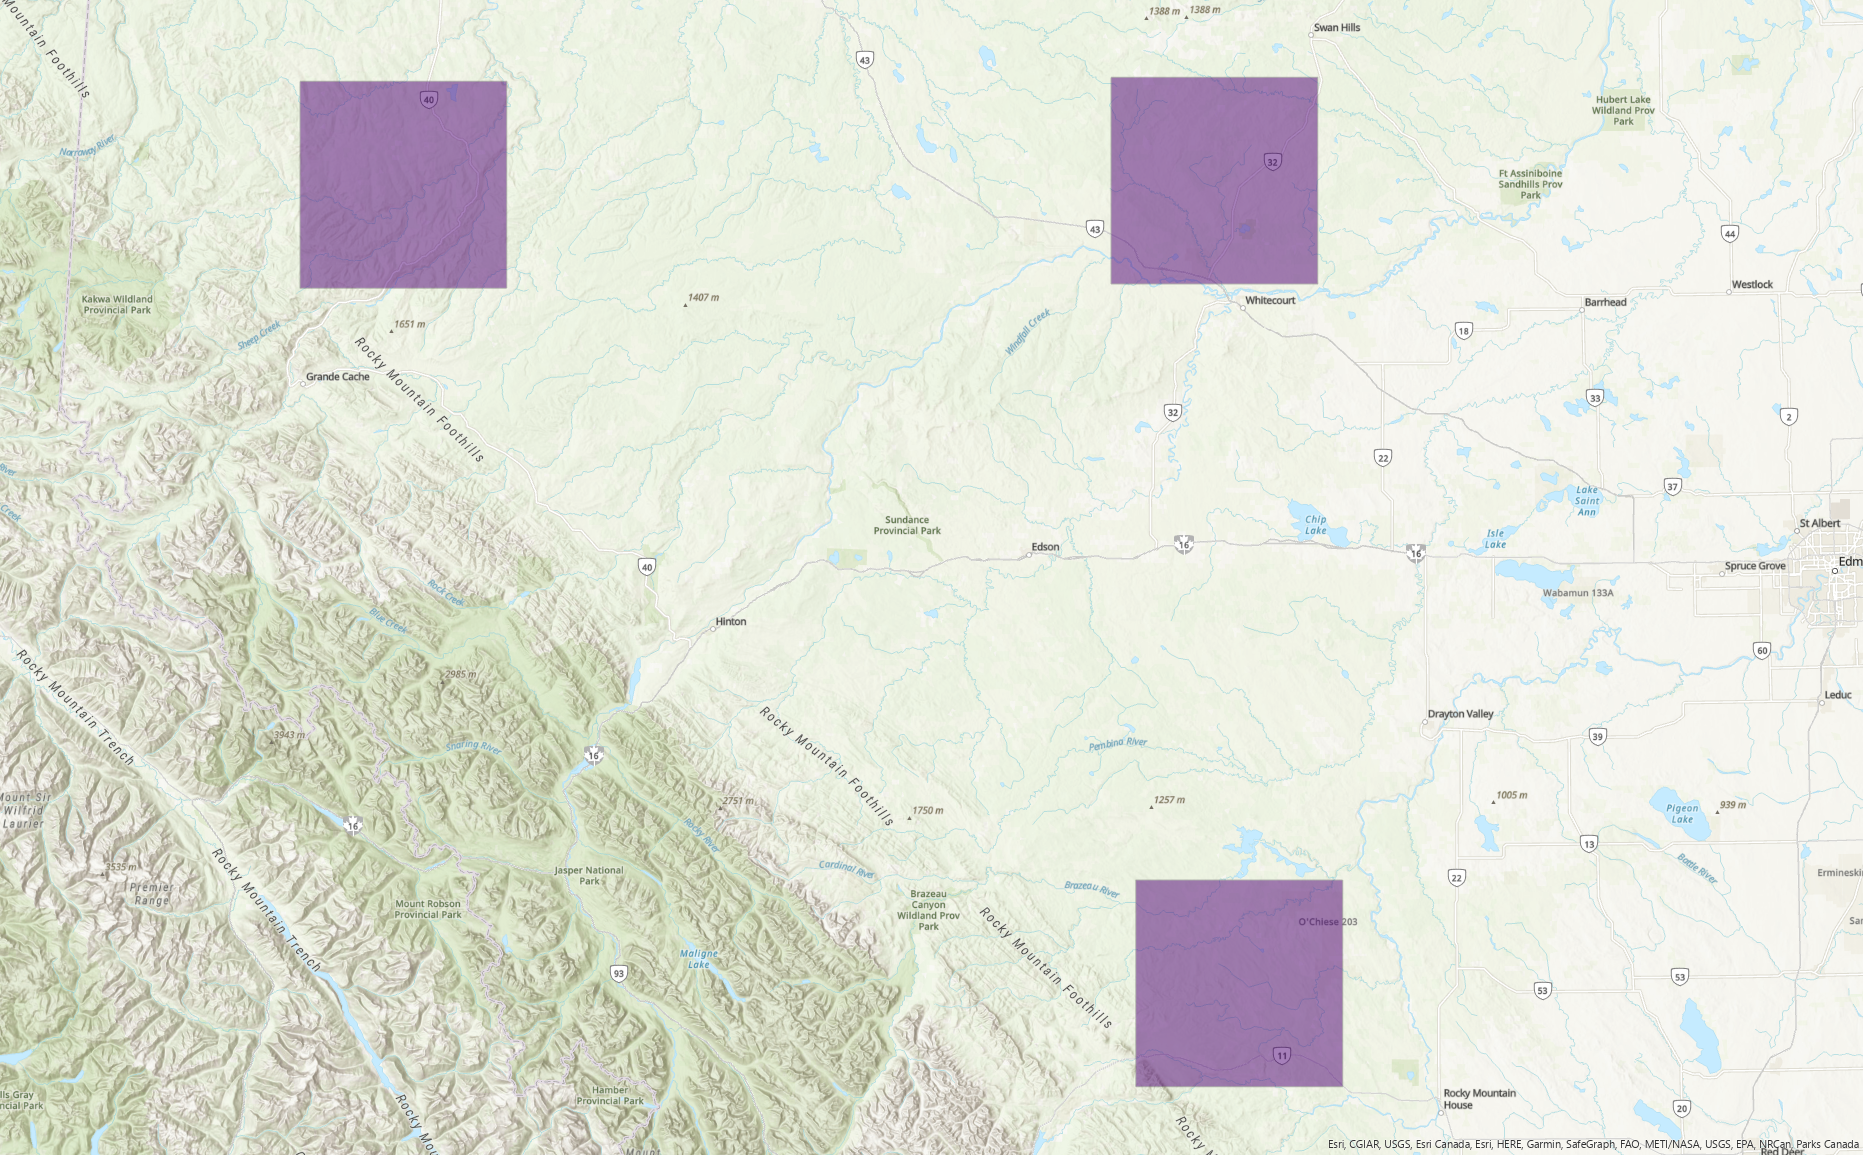
\includegraphics[width=0.8\linewidth]{../graphics/AreasOfInterest} 

}

\caption{50 km by 50 km areas of interest for further investigation.}\label{fig:AoIs}
\end{figure}

As already shown by various authors before, lodgepole pine (Pinus contorta) is the most commonly attacked by MPB, thus, areas where chosen, where lodgepole pine is one of the most dominant species. This information was based on a visual analysis of species classification, how it was in 2019, on a 30 m by 30 m grid. Each resulting pixel is classified as the most dominant tree species within that pixel. Where trees were not the dominant species, the pixel is classified as ``No Tree''. Table \ref{tab:species}shows all species that dominate the area classified within at least one pixel and their corresponding value and NFI codes.

\begin{table}

\caption{\label{tab:species}Value and NFI Code for Species Common Names}
\centering
\begin{tabular}[t]{llll}
\toprule
Value Code & NFI Code & Common Species Name & Scientific Species Name\\
\midrule
0 & NO.TREE & No Trees & \\
2 & ABIE.BAL & Balsam Fir & Abies balsamea\\
3 & ABIE.LAS & Subalpine Fir & Abies lasiocarpa\\
10 & BETU.PAP & White Birch & Betula papyrifera\\
13 & LARI.LAR & Tamarack & Larix laricina\\
\addlinespace
16 & PICE.ENG & Engelmann Spruce & Picea engelmannii\\
17 & PICE.GLA & White Spruce & Picea glauca\\
18 & PICE.MAR & Black Spruce & Picea mariana\\
22 & PINU.BAN & Jack Pine & Pinus banksiana\\
23 & PINU.CON & Lodgepole Pine & Pinus contorta\\
\addlinespace
27 & POPU.BAL & Balsam Poplar & Populus balsamifera\\
29 & POPU.TRE & Trembling Aspen & Populus tremuloides\\
30 & PSEU.MEN & Douglas-Fir & Pseudotsuga menziesii\\
35 & TSUG.HET & Western Hemlock & Tsuga heterophylla\\
\bottomrule
\end{tabular}
\end{table}

The government of Alberta conducts annual Heli-GPS surveys, usually between August 15 and September 15 by flying helicopters at low hight and mapping the GPS locations of detected disturbances in therms of red- and green-attack through observers. These locations have a positional accuracy of +/- 30 m. In most cases only patches consisting of at least 3 trees are recorded. For each of these locations the corresponding cell from the raster data containing the tree species is determined and with a box filter of 5 by 5 the most common tree species for each point can be determined. An example for these buffered GPS locations and the corresponding species data is shown in fig.~\ref{fig:bufferedPointsExample}. This analysis is performed for each of the three areas of interest, both in absolute numbers of pixels within each kernel and relative to the total number of included pixels for each year. It is possible that an area surrounding a GPS location only consists of pixels that have been classified as ``No Tree''. This only means that, in 2019 when the data had been collected, the corresponding 30 by 30 m cell was not predominantlyS covered by trees.

\begin{figure}

{\centering 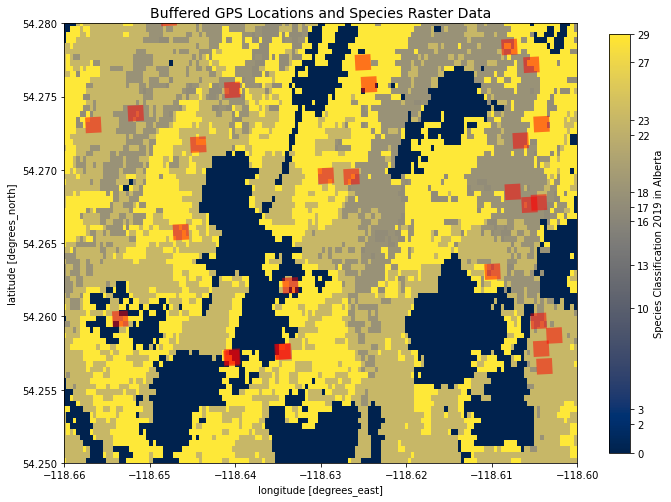
\includegraphics[width=0.8\linewidth]{../graphics/bufferedPointsExample} 

}

\caption{Exemplary buffered GPS locations}\label{fig:bufferedPointsExample}
\end{figure}
\begin{figure}

{\centering 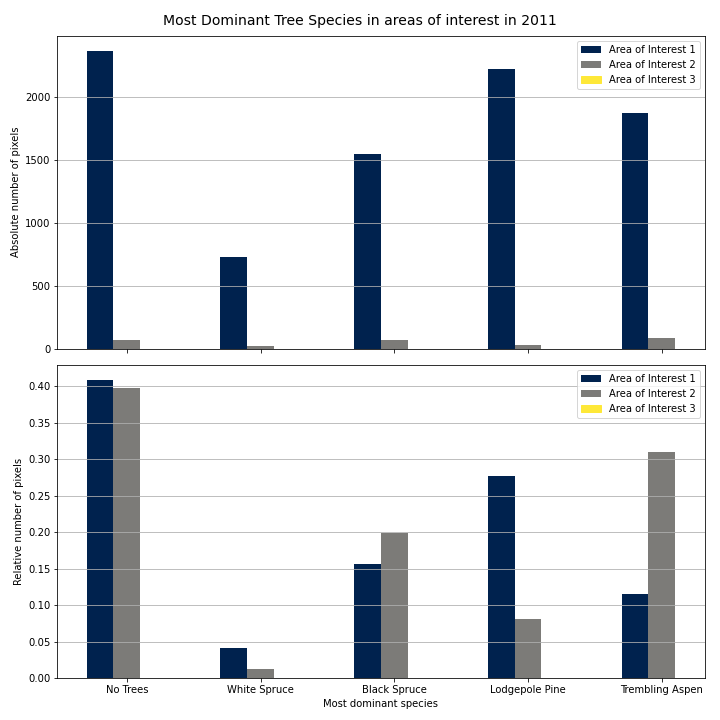
\includegraphics[width=0.8\linewidth]{../graphics/freq_species_11} 

}

\caption{Frequency of tree species within the surrounding area of each MPB survey point for the year 2011.}\label{fig:freqSpecies11}
\end{figure}
\begin{figure}

{\centering 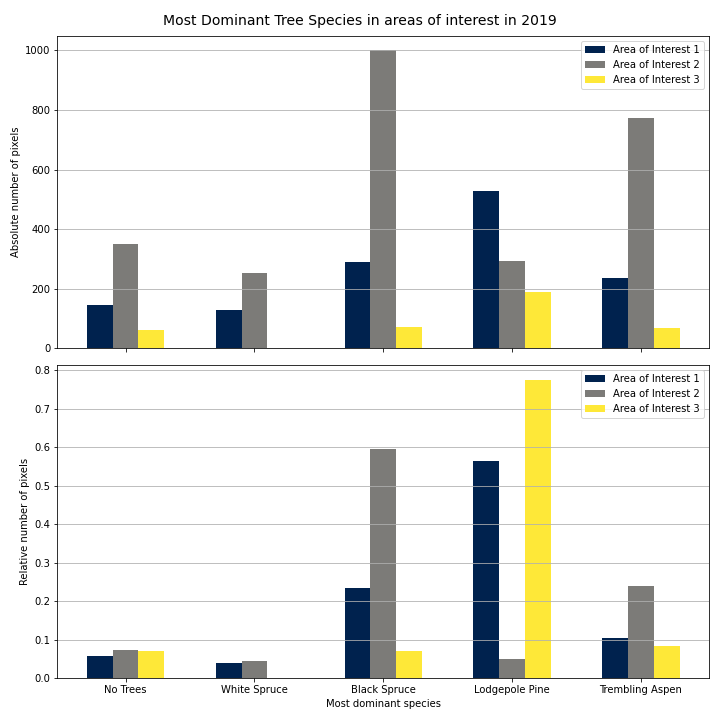
\includegraphics[width=0.8\linewidth]{../graphics/freq_species_19} 

}

\caption{Frequency of tree species within the surrounding area of each MPB survey point for the year 2019.}\label{fig:freqSpecies19}
\end{figure}
\begin{figure}

{\centering 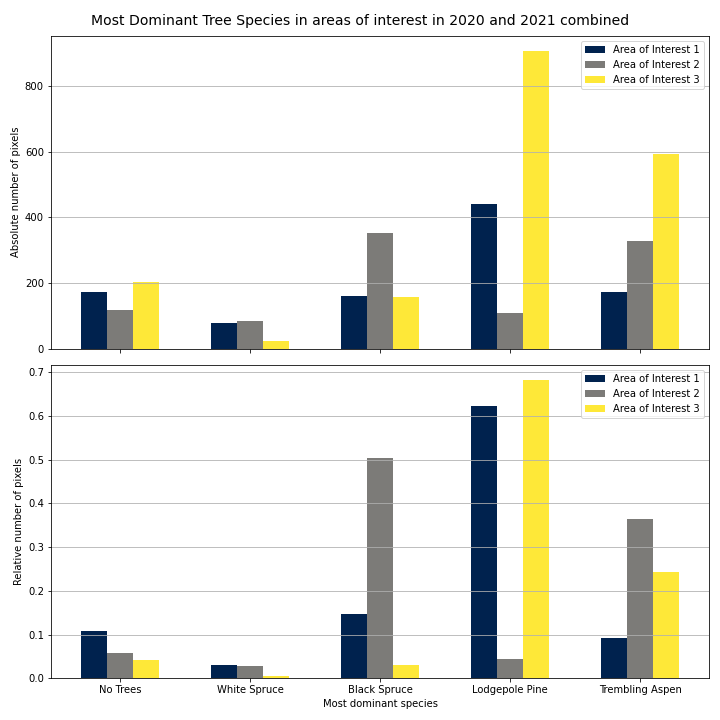
\includegraphics[width=0.8\linewidth]{../graphics/freq_species_20_21} 

}

\caption{Frequency of tree species within the surrounding area of each MPB survey point for the years 2020 and 2021 combined.}\label{fig:freqSpecies20-21}
\end{figure}

The high amount of pixels not dominated by trees in the year 2011 can be explained, when overlaying the GPS points with the species classification in 2018. In many areas where MPB infestation had been an issue in 2011, the trees were harvested by 2019. Each of the areas of interest has similar variance. In the GP and RMH areas, lodgepole pine is the most common species with 36.04 \% and 51.51 \% respectively, while black spruce is most common in the WC area with 34.41 \% and only 13.32 \% LPP. Having similar variances, the most frequent species in the area of GPS locations for red-attack reflect this.

Information on accessibility is based on the road network available through the government of Alberta (Alberta 2021a, 2021b), since all flight locations with the drone need to be accessible from the road for efficient data collection. As the drone has to stay in line of sight, it is not possible to fly far away from the road.

This document was written with bookdown (Xie 2022).

\hypertarget{aereas}{%
\section{Aereas}\label{aereas}}

Here are the areas of Interest for us. The areas are based on detected Mountain Pine Beetle in the years 2011, 2019, 2020, and 2021, and in relatively close distance to at least gravel roads. Based on the total number of trees affected by MPB within each area, the selection have been further narrowed down to the top 50 \% and top 25 \% in orange and re respectively.

\begin{figure}

{\centering 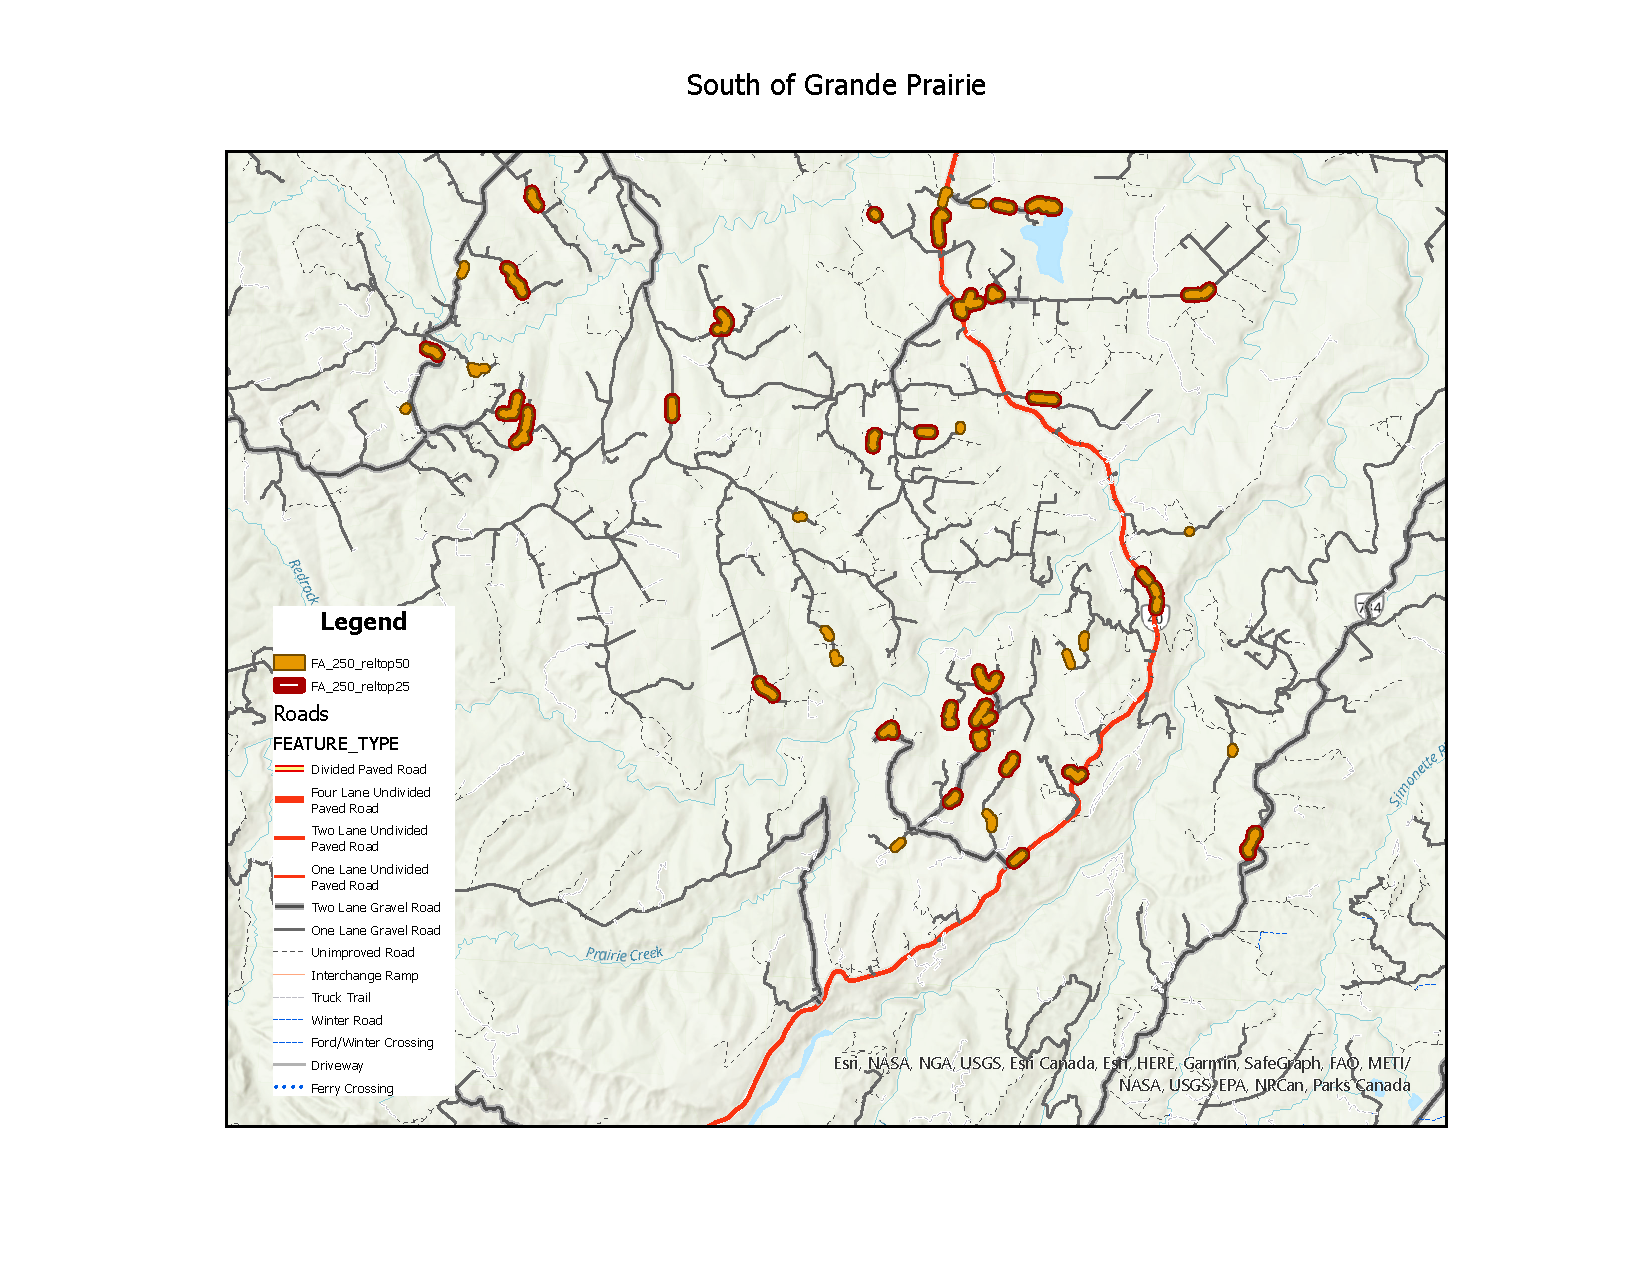
\includegraphics[width=0.8\linewidth]{../graphics/South-of-Grande-Prairie} 

}

\caption{Area South of Grande Prairie}\label{fig:GP}
\end{figure}
\begin{figure}

{\centering 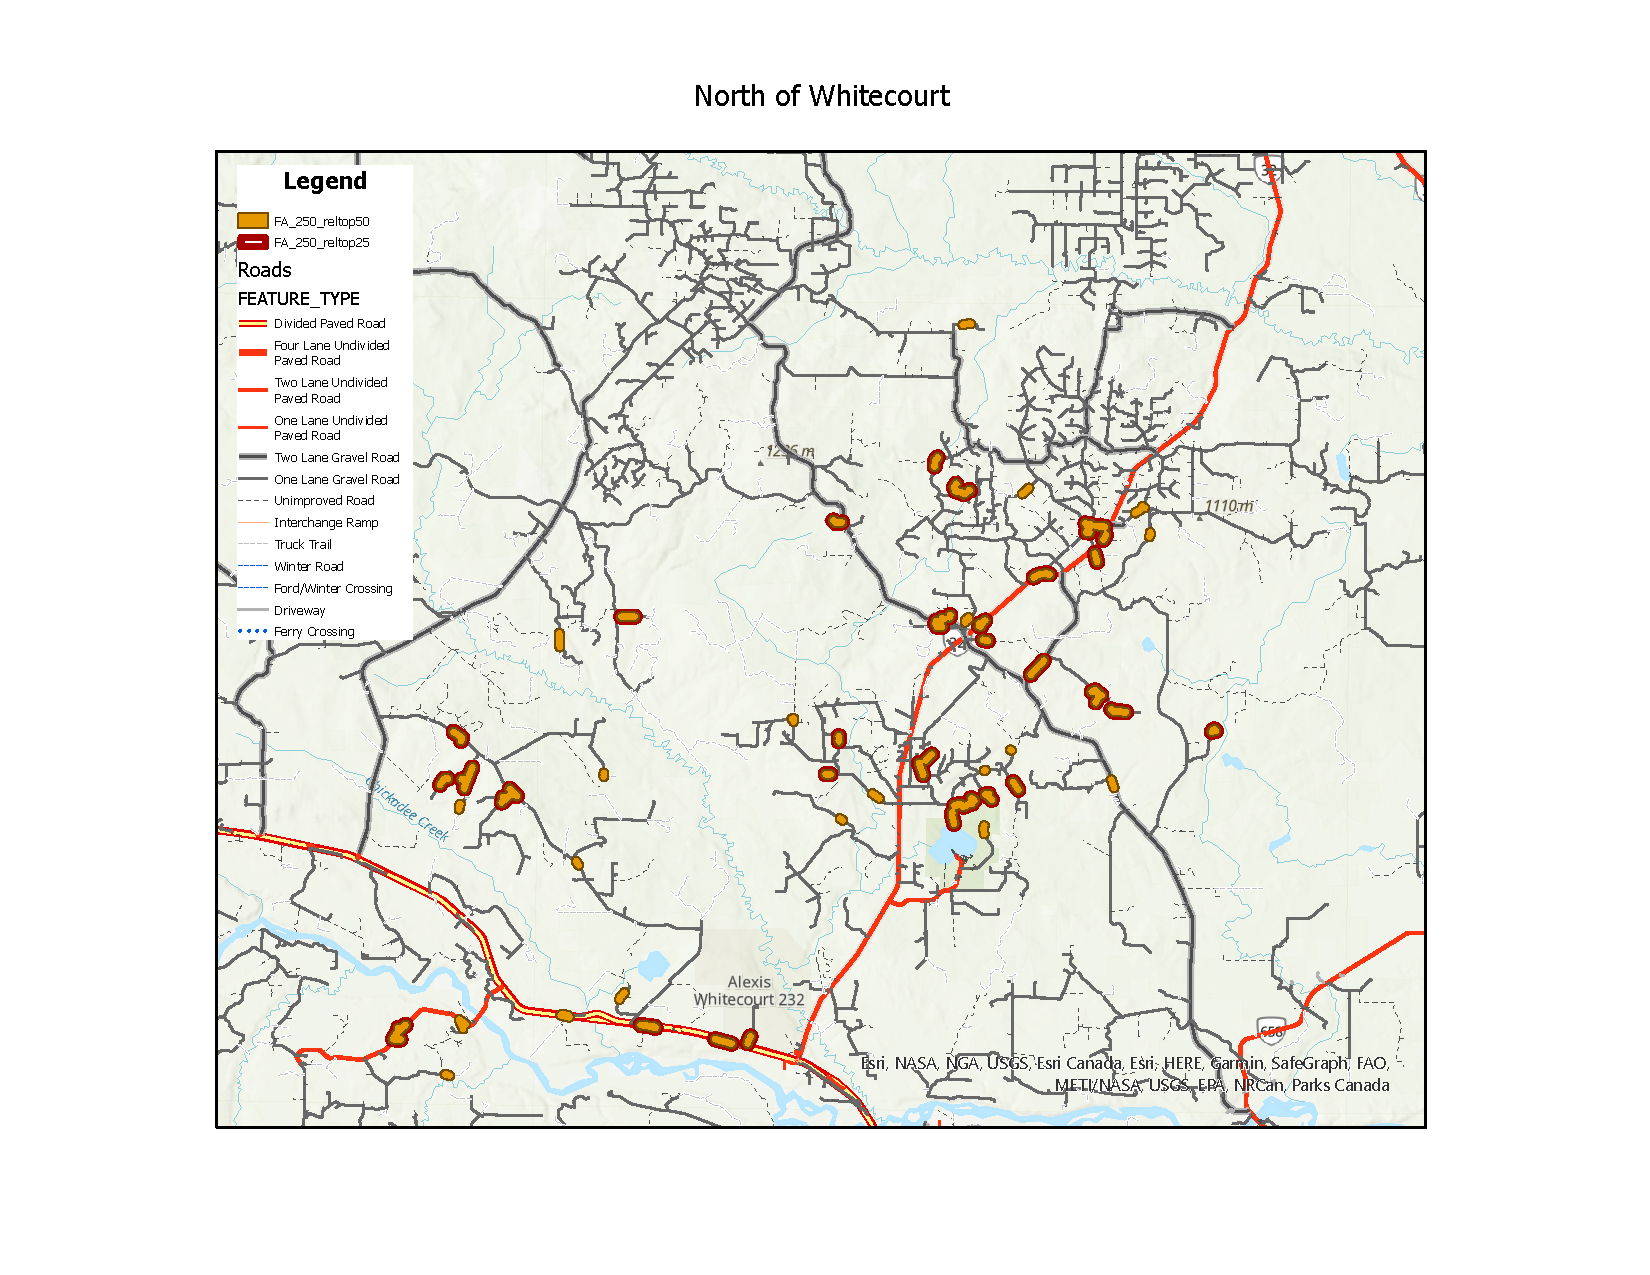
\includegraphics[width=0.8\linewidth]{../graphics/North-of-Whitecourt} 

}

\caption{Area North of Whitecourt}\label{fig:WC}
\end{figure}
\begin{figure}

{\centering 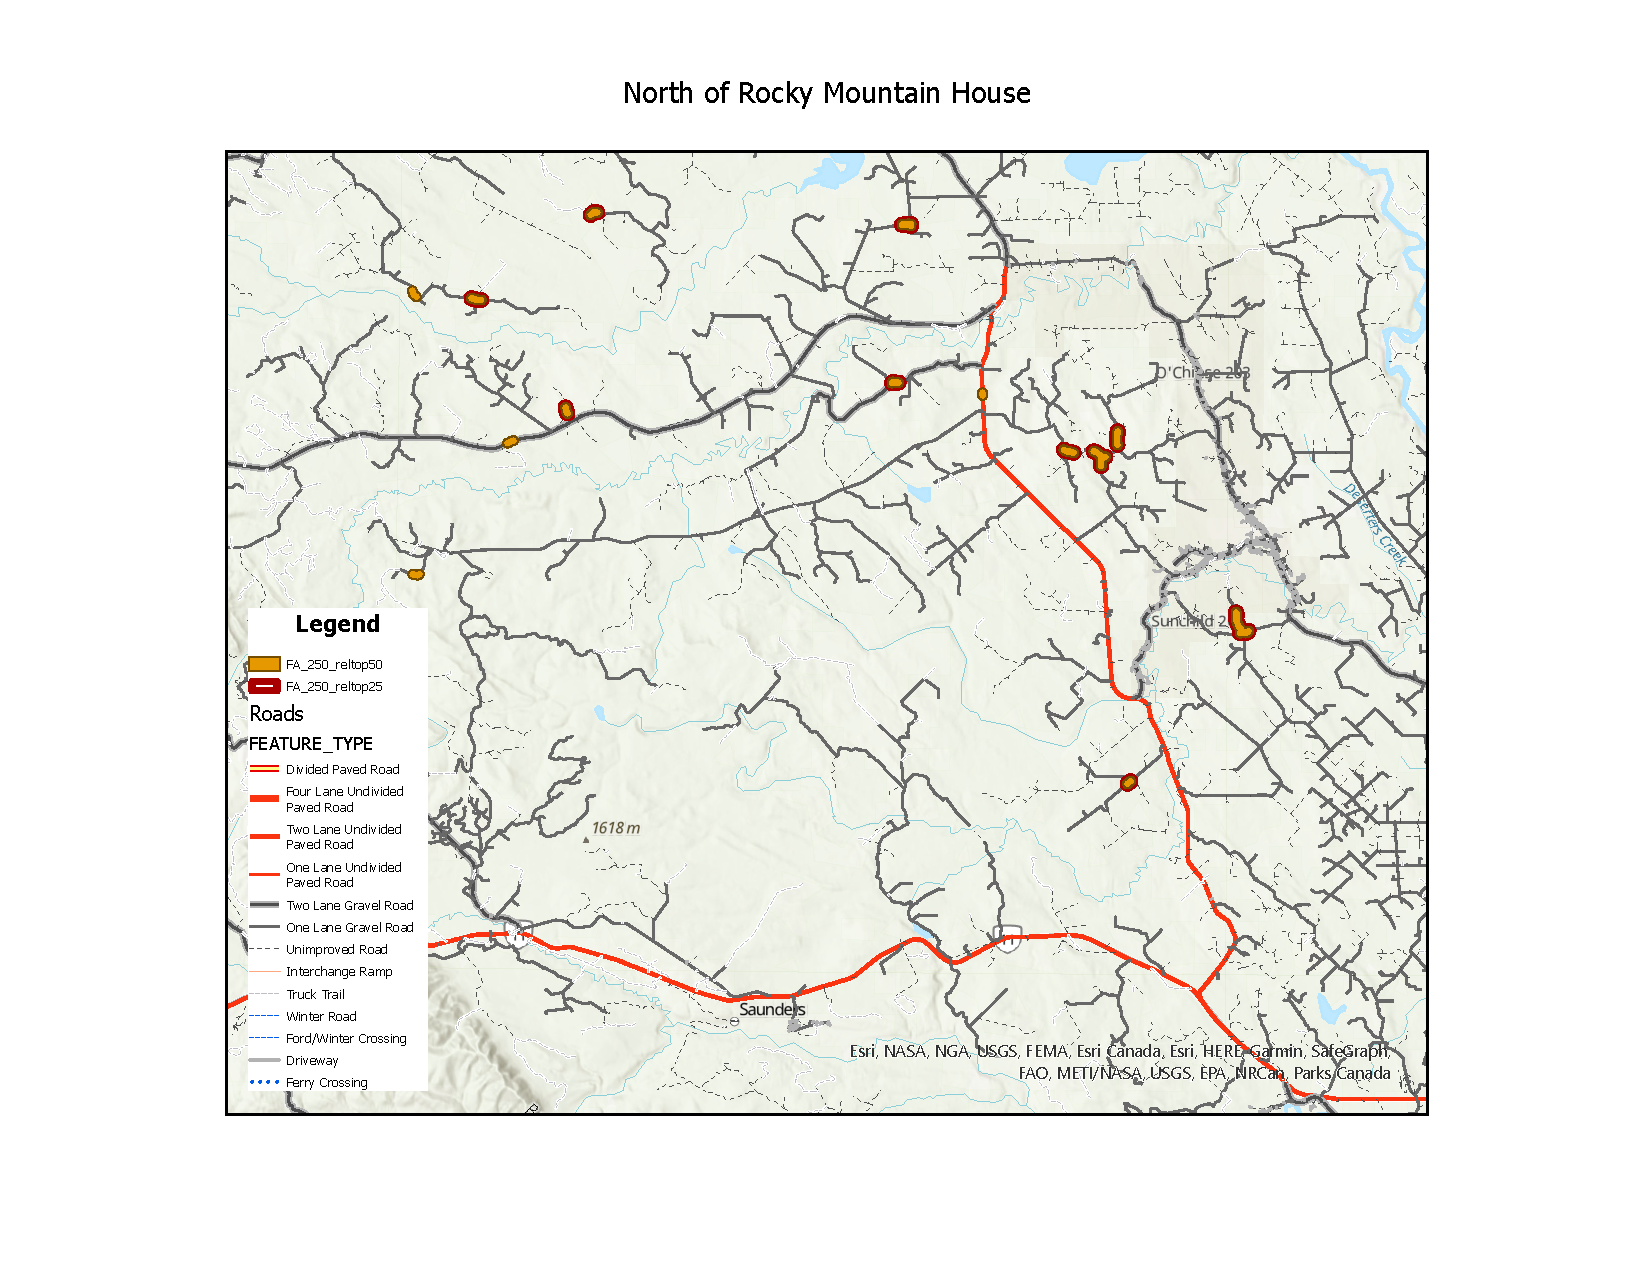
\includegraphics[width=0.8\linewidth]{../graphics/North-of-RMH} 

}

\caption{Area North-West of Rocky Mountain House}\label{fig:RMC}
\end{figure}

\hypertarget{references}{%
\section{References}\label{references}}

\hypertarget{references}{}

\hypertarget{refs}{}
\begin{CSLReferences}{1}{0}
\leavevmode\vadjust pre{\hypertarget{ref-GravelRoad2021}{}}%
Alberta, Government of. 2021a. {``Layer: {Gravel Road} ({20k}) ({ID}: 23).''} May 26, 2021. \url{https://geospatial.alberta.ca/titan/rest/services/utility/access/MapServer/23}.

\leavevmode\vadjust pre{\hypertarget{ref-PavedRoad2021}{}}%
---------. 2021b. {``Layer: {Paved Road} ({20k}) ({ID}: 14).''} June 25, 2021. \url{https://geospatial.alberta.ca/titan/rest/services/utility/access/MapServer/14}.

\leavevmode\vadjust pre{\hypertarget{ref-mitchellFallRateLodgepole1998}{}}%
Mitchell, Russel G., and Haiganoush K. Preisler. 1998. {``Fall {Rate} of {Lodgepole Pine Killed} by the {Mountain Pine Beetle} in {Central Oregon}.''} \emph{Western Journal of Applied Forestry} 13 (1): 23--26. \url{https://doi.org/10.1093/wjaf/13.1.23}.

\leavevmode\vadjust pre{\hypertarget{ref-schoennagelEffectsMountainPine2012}{}}%
Schoennagel, Tania, Thomas T. Veblen, José F. Negron, and Jeremy M. Smith. 2012. {``Effects of {Mountain Pine Beetle} on {Fuels} and {Expected Fire Behavior} in {Lodgepole Pine Forests}, {Colorado}, {USA}.''} \emph{PLOS ONE} 7 (1): e30002. \url{https://doi.org/10.1371/journal.pone.0030002}.

\leavevmode\vadjust pre{\hypertarget{ref-wulderRemoteSensingSurvey2005}{}}%
Wulder, Michael A., Joanne C. White, and Caren C. Dymond. 2005. \emph{Remote Sensing in the Survey of Mountain Pine Beetle Impacts: Review and Recommendations}. Information Report, BC-X-401. {Victoria, B.C}: {Pacific Forestry Centre}.

\leavevmode\vadjust pre{\hypertarget{ref-R-bookdown}{}}%
Xie, Yihui. 2022. \emph{Bookdown: Authoring Books and Technical Documents with r Markdown}.

\end{CSLReferences}

\end{document}
